


  Suppose $m\angle ACB=90^\circ$ and 
$m\angle ACD=m\angle BCD$.  If $AB=10$ and $AC=CB$, then which of the following cannot be a value for $BD$?
 \begin{center}
 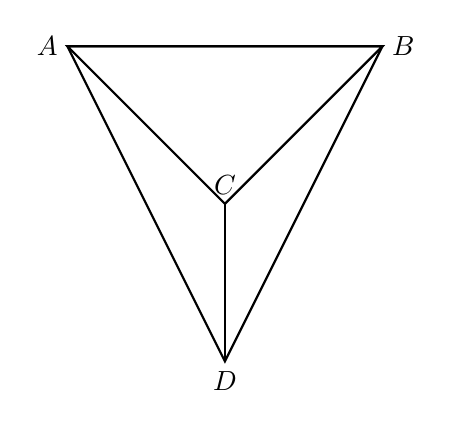
\begin{tikzpicture}
 
 \draw (0,0) --(2,-2)--(4,0)--cycle  [thick,-,>=latex];
 \draw (0,0) --(2,-4)--(4,0)--cycle  [thick,-,>=latex];
 \draw (2,-2) --(2,-4)  [thick,-,>=latex];
  \draw node[above] at (2,-2) {$C$};
  \draw node[left] at (0,0) {$A$};
  \draw node[right] at (4,0) {$B$};
  \draw node[below] at (2,-4) {$D$};    
  
   
  
 
   
\end{tikzpicture}
\end{center}




\ifsat
	\begin{enumerate}[label=\Alph*)]
		\item   $7$%
		\item $9$ 
		\item  $10$ 
		\item  $11$ 
	\end{enumerate}
\else
\fi

\ifacteven
	\begin{enumerate}[label=\textbf{\Alph*.},itemsep=\fill,align=left]
		\setcounter{enumii}{5}
		\item   $7$%
		\item    $8$   
		\item $9$ 
		\addtocounter{enumii}{1}
		\item  $10$ 
		\item  $11$ 
	\end{enumerate}
\else
\fi

\ifactodd
	\begin{enumerate}[label=\textbf{\Alph*.},itemsep=\fill,align=left]
		\item   $7$%
		\item    $8$   
		\item $9$ 
		\item  $10$ 
		\item  $11$ 
	\end{enumerate}
\else
\fi

\ifgridin
   $7$%
		
\else
\fi

